\documentclass[10pt,xcolor=pdflatex]{beamer}
\usepackage{newcent}
\usepackage[utf8]{inputenc}
%\usepackage[czech]{babel}
\usepackage{hyperref}
\usepackage{fancyvrb}
\usetheme{FIT}

%%%%%%%%%%%%%%%%%%%%%%%%%%%%%%%%%%%%%%%%%%%%%%%%%%%%%%%%%%%%%%%%%%
\title[TSD Analyser]{Obhajoba semestrálneho projektu}

\author[]{Dušan Želiar}

\institute[]{Vysoké učení technické v Brně, Fakulta informačních technologií\\
Bo\v{z}et\v{e}chova 1/2. 612 66 Brno - Kr\'alovo Pole\\
xzelia00@stud.fit.vutbr.cz}

\date{21.1, 2019}
%\date{\today}
%\date{} % bez data

%%%%%%%%%%%%%%%%%%%%%%%%%%%%%%%%%%%%%%%%%%%%%%%%%%%%%%%%%%%%%%%%%%

\begin{document}

\frame[plain]{\titlepage}
\begin{frame}\frametitle{Syntéza stromových štruktúr z reálnych dát}
Zameranie na automatizovanú \textbf{analýzu} závislostí \textbf{vzoriek} dát
\begin{itemize}
	\item{\textit{Vzory} stromových štruktúr 
	}
	\item{\textit{Hodnoty} uzlov 
	}	
\end{itemize}
Výsledkom je \textbf{predpis pre generovanie} testovacích dát
	\begin{itemize}
		\item{\textit{Štruktúrou aj významom} podobné reálnym vzorkám
		}	
	
\end{itemize}
\end{frame}
\begin{frame}\frametitle{Spolupráca modulov Testos}
\begin{figure*}\centering
	\centering
	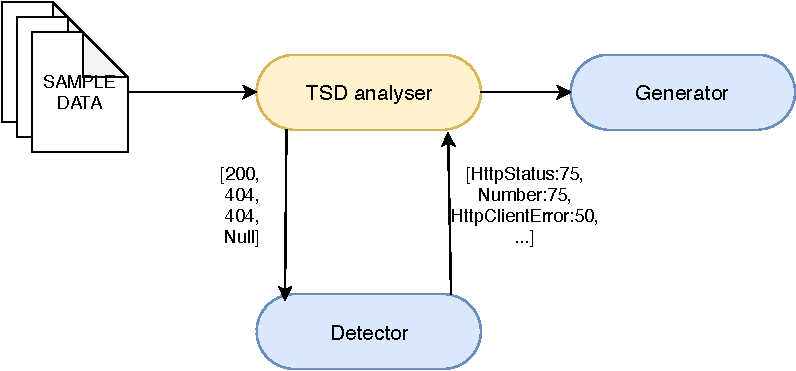
\includegraphics[width=3.0in,keepaspectratio]{img/testos_components.pdf}\\[1pt]
	\caption{Sémantickú analýzu množiny hodnôt vykonáva komponenta Detector }
\end{figure*} 
\\
\\

\end{frame}
\begin{frame}\frametitle{Algoritmus tvorby abstraktného stromu č.1}
\begin{figure*}\centering
	\centering
	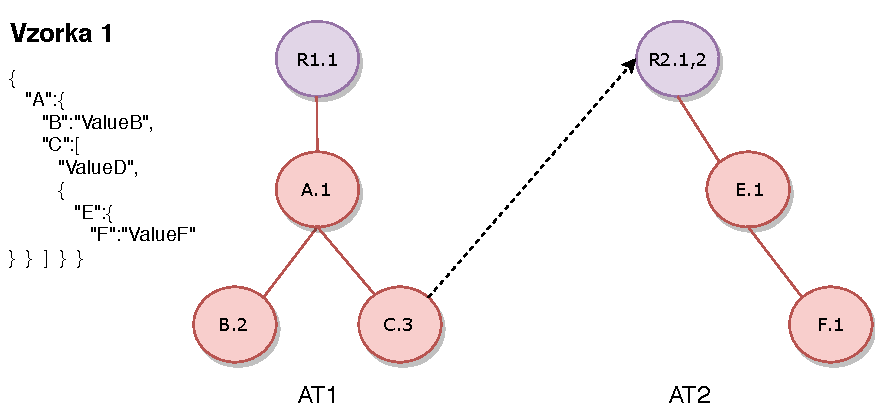
\includegraphics[width=3.5in,keepaspectratio]{img/slide_example1.pdf}\\[1pt]
\end{figure*} 	
Uzly \textit{AN} stromu \textit{AT} nesú tri typy informácií
\begin{enumerate}
	\item{\textbf{Object}: Uzol obsahuje nezoradenú množinu AN uzlov. 
	}	
	\item{\textbf{Value}: Uzol obsahuje konkrétnu hodnotu. 
	}	
	\item{\textbf{Array}: Uzol obsahuje množinu referencií na AT. 
	}		
\end{enumerate}
\end{frame}
\begin{frame}\frametitle{Algoritmus tvorby abstraktného stromu č.2}
	\begin{figure*}\centering
		\centering
		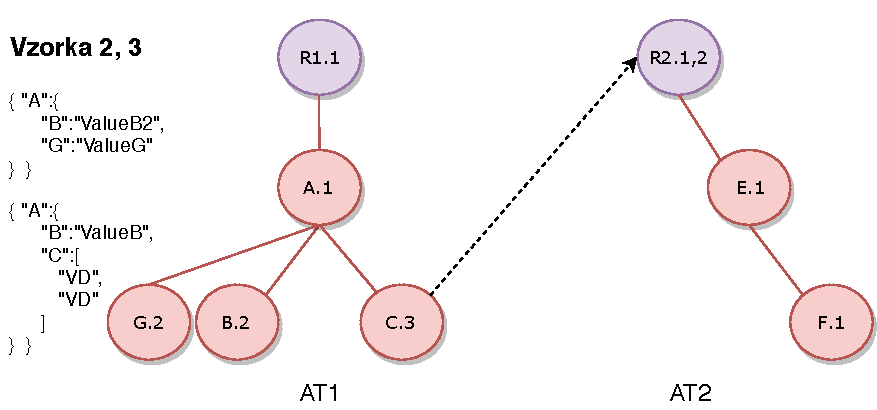
\includegraphics[width=3.5in,keepaspectratio]{img/slide_example2.pdf}\\[1pt]
	\end{figure*} 
\begin{table}[hbt]
	\centering
	\label{alg_example3_tab}
	\begin{tabular}{|p{1.8cm}|p{9cm}|}
		\hline
		\textbf{Množina} & \textbf{Prvky} \\ \hline
		AT1 vzory & 	\(ATP1 = \{R1.1, A.1, B.2, C.3\},\)\\  
		& \(ATP4 = \{R1.1, A.1, B.2, G.2\}\)   \\ \hline 
		AT2 vzory & 	\(ATP2 = \{R2.2\}, ATP3 = \{R2.1, E.1, F.2 \}  \)   \\ \hline		
		Pattern &\(CP1 = \{ATP1, ATP2, ATP3\}, CP2 = \{ATP4\},\)\\ 
		& \(CP3 = \{ATP1, ATP2\}  \)\\ \hline
		DataStore & 	\(B.2 = \{"ValueB", "ValueB2", "ValueB"\},\)\\
		&  \(R2.2 = \{"ValueD", "VD", "VD"\}, F.2 = \{"ValueF"\}  \)   \\ \hline								
		
	\end{tabular}
	\caption{Tabuľka zobrazujúca stav množín po spracovaní tretieho vzorku dát}
\end{table} 
\end{frame}
\begin{frame}\frametitle{Aktuálny stav}
\begin{itemize}
	\item{Naštudované princípy testovania založeného na dátach
	}
	\item{Analýza požiadaviek pre syntézu umelých testovacích dát  
	}
	\item{Návrh algoritmu detekcie štruktúry vzoriek
	}			
\end{itemize}
\end{frame}
\begin{frame}\frametitle{Budúca práca}
\begin{itemize}
	\item{Definícia rozhrania komponenty
	}
	\item{Návrh vizualizácie abstraktného stromu
	}	
	\item{Implementácia nástroja a grafického rozhrania
	}
	\item{Integračné testovanie komponenty
	}				
\end{itemize}
\end{frame}

\bluepage{Ďakujem za pozornosť}

\end{document}
